\documentclass[10pt]{beamer}
\usepackage[UTF8]{ctex}
\usepackage{outlines}
\usepackage{hyperref}
\usepackage{minted}
\usepackage{booktabs}
\usemintedstyle{xcode}
\usepackage{tcolorbox}
\tcbuselibrary{minted}

\setminted{
    fontfamily=helvetica
}
\AtBeginSection[]{
  \begin{frame}
  \tableofcontents[currentsection, hideothersubsections]
  \end{frame}
}

\ifx\pdfoutput\undefined
% we are running LaTeX, not pdflatex
\usepackage{graphicx}
\else
% we are running pdflatex, so convert .eps files to .pdf
\usepackage{graphicx}
\usepackage{epstopdf}
\fi

%--------------------------------------------------------
% NOTE: 1) This is an UNOFFICIAL LaTeX beamer style for 
%           Beihang University.
%       2) This is not exactly a beamer style, rather
%           it contains two LaTeX files to be inserted 
%           in the slides' source file.
%       3) These files are based on Edward Hartley's work
%   <http://www-control.eng.cam.ac.uk/Main/EdwardHartley>
%       4) Complaints or suggestions are always welcome.
%
% Xiaoke Yang (das.xiaoke@hotmail.com)
% Wed 15 Jun 11:02:17 CST 2016
%--------------------------------------------------------


%--------------------------------------------------------
% Set up the Beihang University Colours for use with
% xcolor
%--------------------------------------------------------

% Blue palette
\definecolor{coreBlue}{rgb}{0.02 0.30588 0.64706} %#254aa5


%--------------------------------------------------------
% NOTE: 1) This is an UNOFFICIAL LaTeX beamer style for 
%           Beihang University.
%       2) This is not exactly a beamer style, rather
%           it contains two LaTeX files to be inserted 
%           in the slides' source file.
%       3) These files are based on Edward Hartley's work
%   <http://www-control.eng.cam.ac.uk/Main/EdwardHartley>
%       4) Complaints or suggestions are always welcome.
%
% Xiaoke Yang (das.xiaoke@hotmail.com)
% Wed 15 Jun 11:02:17 CST 2016
%--------------------------------------------------------

%--------------------------------------------------------
% Require tikz to do some text positioning
%--------------------------------------------------------
\usepackage{tikz}

%--------------------------------------------------------
% Use Helvetica rather than Computer Modern Sans Serif
% Comment this out if you prefer Computer Modern
%\usepackage{times}
%--------------------------------------------------------
%\usepackage{helvet}

%--------------------------------------------------------
% If you wish to use Arial, and have the winfonts package
% correctly installed uncomment the following to make the
% default sans serif font Arial
%--------------------------------------------------------
%\usepackage{winfonts}
%\usepackage[T1]{fontenc}
%\renewcommand{\sfdefault}{arial}
%--------------------------------------------------------

%--------------------------------------------------------
% Get rid of the navigation bar 
%--------------------------------------------------------
\beamertemplatenavigationsymbolsempty

%--------------------------------------------------------
% Set the files corresponding to the University crests
% here
%--------------------------------------------------------
% Crest with blue text
\newcommand{\beihangcrestblack}{beihangbeamerstyle/beihang-pantone}

% Crest with white text
\newcommand{\beihangcrestwhite}{beihangbeamerstyle/beihang-rev-pantone}
%--------------------------------------------------------

%--------------------------------------------------------
% Define how the page counter will be displayed on slides
%--------------------------------------------------------
\newcommand{\footlinepagecounter}%
	{\insertframenumber{}/\inserttotalframenumber}
%--------------------------------------------------------

%--------------------------------------------------------
% Set up some lengths
%--------------------------------------------------------
% A paper width for the footline
\newlength{\halfpaperwidth}

% The left margin
\newlength{\headingleftmargin}
% Paper width minus margins
\newlength{\headingwidthminusmargins}
% Height of the heading block
\newlength{\headingheight}
% Height of the footer block
\newlength{\footerheight}

% The height for the titlepageheader in the title page
\newlength{\titlepageheaderheight}
% The height for the footer in the title page
\newlength{\titlepagefooterheight}
% The height for the main title block
\newlength{\titlepagemaintitleblockheight}
% The height for the subtitle block
\newlength{\titlepagesubtitleblockheight}
% The height for the name and date block
\newlength{\titlepagenamedateblockheight}
% The height for the institution block
%\newlength{\titlepageinstitutionheight}

% The lengths for spacing between name and date
\newlength{\titlepagespaceundername}
\newlength{\titlepagespaceunderdate}

% The length for the light blue thin bar


\setlength{\headingleftmargin}{0.05573\paperwidth}
\setlength{\headingwidthminusmargins}{\paperwidth}
\addtolength{\headingwidthminusmargins}{-\headingleftmargin}
\setlength{\headingheight}{0.1459\paperheight}
\setlength{\footerheight}{0.09017\paperheight}

\setlength{\titlepageheaderheight}{0.2361\paperheight}
\setlength{\titlepagefooterheight}{0.1459\paperheight}
\setlength{\titlepagemaintitleblockheight}{0.2361\paperheight}
\setlength{\titlepagesubtitleblockheight}{0.1459\paperheight}
\setlength{\titlepagenamedateblockheight}{0.2361\paperheight}
%\setlength{\titlepageinstitutionheight}{0.95cm}

\setlength{\titlepagespaceundername}{16pt}
\setlength{\titlepagespaceunderdate}{8pt}

%--------------------------------------------------------

%--------------------------------------------------------
% Set up the Beihang University blue scheme for use
% with beamer
%--------------------------------------------------------

% Define colour names
\setbeamercolor{coreBlue}{bg=coreBlue, fg=white}

% Set element colours
\setbeamercolor{subtitle}{fg=white}
\setbeamercolor{titlepageheader}{bg=white,fg=black}
\setbeamercolor{titlepagefooter}{bg=white,fg=black}
\setbeamercolor{block title}{bg=white, fg=coreBlue}
\setbeamercolor{structure}{bg=white, fg=coreBlue}
% \setbeamercolor{alerted text}{fg=darkOrange}


%--------------------------------------------------------
% Set font sizes
%--------------------------------------------------------
\setbeamerfont{frametitle}{size=\large,series=\bfseries}
\setbeamerfont{title}{size=\large,series=\bfseries}
\setbeamerfont{author}{size=\normalsize}
\setbeamerfont{date}{size=\scriptsize}
\setbeamerfont{subtitle}{size=\footnotesize,series=\bfseries}
\setbeamerfont{block title}{size=\normalsize,series=\bfseries}
\setbeamerfont{structure}{size=\normalsize,series=\bfseries}

\setbeamertemplate{itemize item}{\scriptsize\raise1.25pt\hbox{\textbullet}}
\setbeamertemplate{itemize subitem}{\scriptsize\raise1.25pt\hbox{\textbullet}}
\setbeamertemplate{itemize subsubitem}{\scriptsize\raise1.25pt\hbox{\textbullet}}


%-----------------------------------------------------
% Define frame title drawing
%-----------------------------------------------------
\setbeamertemplate{frametitle}
{%
  \nointerlineskip
  \begin{beamercolorbox}[wd=\paperwidth,leftskip=\headingleftmargin]{coreBlue}
    \vskip1pt%
    \tikz{\node[minimum height=\headingheight, inner sep=0cm, text width= \headingwidthminusmargins, text badly ragged]{\usebeamerfont{frametitle}\insertframetitle\\\normalsize\it\insertframesubtitle};}
  \end{beamercolorbox}%
}

%-----------------------------------------------------
% Define footline drawing
%-----------------------------------------------------
\setbeamertemplate{footline}
{%
 \setlength{\halfpaperwidth}{0.5\paperwidth}
 \addtolength{\halfpaperwidth}{1pt}
 \leavevmode
 \begin{beamercolorbox}[sep=0pt,wd=\halfpaperwidth, leftskip=\headingleftmargin,right]{coreBlue}
 \tikz{\node[minimum height=\footerheight, inner sep=0cm]{\footlinepagecounter};}%
 \end{beamercolorbox}
 \hskip-1.5pt%
 \begin{beamercolorbox}[sep=0pt,wd=\halfpaperwidth, leftskip=\headingleftmargin, right,rightskip=\headingleftmargin]{coreBlue}
 \tikz{\node[minimum height=\footerheight, inner sep=0cm]{\includegraphics[width=0.25\paperwidth]{\beihangcrestwhite}};}%
 \end{beamercolorbox}%
}


%-----------------------------------------------------
% Define BEIHANG title page
%-----------------------------------------------------
\setbeamertemplate{title page}
{%
\begin{beamercolorbox}[sep=0cm,right,wd=\paperwidth,ht=\titlepageheaderheight,rightskip=\headingleftmargin]{titlepageheader}
\includegraphics[width=0.3820\paperwidth]{\beihangcrestblack}
\vskip0.2361\titlepageheaderheight
\end{beamercolorbox}
\begin{beamercolorbox}[left,leftskip=\headingleftmargin,wd=\paperwidth,ht=\titlepagemaintitleblockheight]{coreBlue}
\tikz{\node[inner sep=0cm, text width=\paperwidth, minimum height=\titlepagemaintitleblockheight,text badly ragged]{\usebeamerfont{title}\inserttitle};}%
\end{beamercolorbox}%
\nointerlineskip%
\vskip-1pt%
\begin{beamercolorbox}[left,leftskip=\headingleftmargin,wd=\paperwidth,ht=\titlepagesubtitleblockheight]{coreBlue}
\tikz{\node[inner sep=0cm, text width=\paperwidth, minimum height=\titlepagesubtitleblockheight, text badly ragged]{\usebeamerfont{subtitle}\usebeamercolor[fg]{subtitle}\insertsubtitle};}%
\end{beamercolorbox}%
\nointerlineskip%
\vskip-1pt%
\begin{beamercolorbox}[left,leftskip=\headingleftmargin,wd=\paperwidth,ht=\titlepagenamedateblockheight]{coreBlue}
      \usebeamerfont{author}\insertauthor\\
      \vskip\titlepagespaceundername%
      \usebeamerfont{date}\insertdate
      \vskip\titlepagespaceunderdate%
    \end{beamercolorbox}%
\begin{beamercolorbox}[left,leftskip=\headingleftmargin,wd=\paperwidth,ht=\titlepagefooterheight]{titlepagefooter}
\end{beamercolorbox}
}


\title{Python入门(三)}
\author{张博涵\\
北京航空航天大学经济管理学院 (\texttt{zhangbohan@buaa.edu.cn})}
\date{\today}


\begin{document}

\begin{frame}
    \maketitle
\end{frame}


\begin{frame}
    \frametitle{Contents}

    \tableofcontents

\end{frame}


\section{条件语句}

\begin{frame}[fragile]
\frametitle{条件语句 - if else}

\begin{tcblisting}{listing only, title = Syntax, minted language=python}
if condition1:
    expr1
elif condition2:
    expr2
elif ...
else:
    expr
\end{tcblisting}

\begin{itemize}
    \item 必须包含if语句,else与elif都是可选的;
    \item condition处的条件必须是布尔型或者可以转换为布尔型;
    \item 当condition为True时,执行对应的expr,然后跳出该条件结构。
\end{itemize}
\end{frame}


\begin{frame}
    \frametitle{比较运算符}

    \begin{table}
        \caption{比较运算符}
        \begin{tabular}{ll} \\ \toprule
            符号 & 含义 \\ \midrule
            <, > & 小于, 大于 \\
            <=, >= & $\leq, \geq$ \\
            == & 相等 \\
            != & $\neq$ \\
            is & 是否完全相等或指向同一对象 \\
            in & 是否被包含 \\\bottomrule
        \end{tabular}
    \end{table}
    \begin{itemize}
        \item 不仅是数字之间可以进行比较,其他类型也可以进行比较,不过比较的形式取决于具体规则和实现的方法。
    \end{itemize}
\end{frame}


\begin{frame}
    \frametitle{逻辑运算符}

    \begin{itemize}
        \item 逻辑运算符用于计算Bool值表达式
    \end{itemize}
    \begin{table}
        \caption{逻辑运算符}
        \begin{tabular}{lll} \toprule
            符号 & 含义 & 示例 \\ \midrule
            not & 非 & \mintinline{python}{not True} \\
            and & 与 & \mintinline{python}{True and True} \\
            or & 或 & \mintinline{python}{True or False} \\ 
            \& | \textasciicircum & 位操作符 & 不建议使用 \\ 
            \bottomrule
    \end{tabular}
    \end{table}

    \begin{itemize}
        \item and 以及 or 都是短路运算,即当运算的结果确定时,后面的表达式不再计算
        \item 可以通过多个逻辑运算以及比较运算符的组合形成复杂的逻辑表达式,但需要注意运算符的优先级,如果不确定,加括号总没错
    \end{itemize}

\end{frame}

\begin{frame}
    \frametitle{运算符的优先级}

    运算符遵循下表的由高到低的优先级
    \begin{figure}
    \centering
    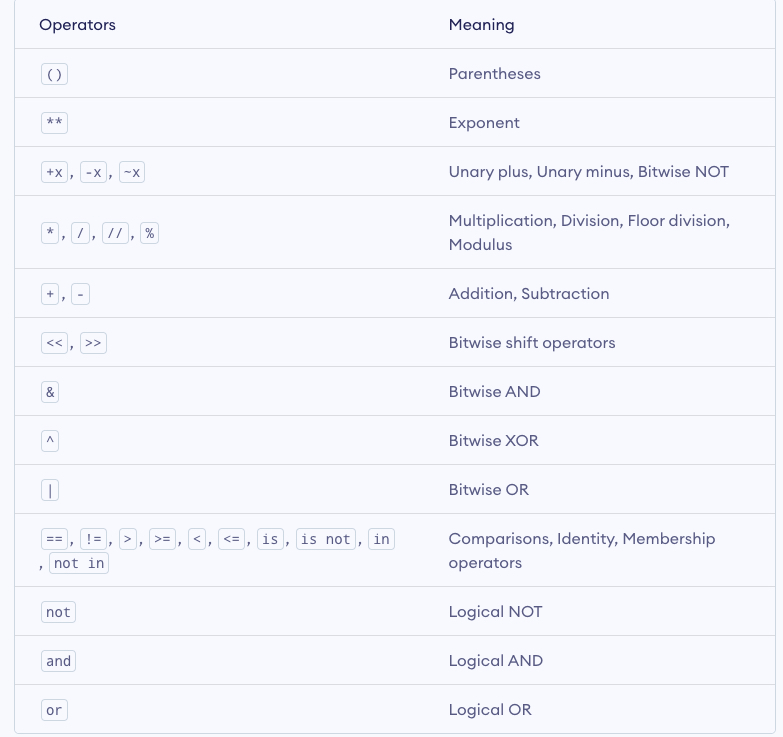
\includegraphics[width=0.6\textwidth]{figures/python_operator.jpg}
    \end{figure}

\end{frame}

\begin{frame}
    将表达式或变量放入到if语句的condition中,若结果不是布尔型,则自动转换成布尔型,因此需要了解将任意类型转换为布尔型的规则
    \frametitle{Boolean 类型转换}
    \begin{block}{数字}
        \mintinline{python}{bool(num)} 等同于 \mintinline{python}{num != 0}
    \end{block}
    \begin{block}{序列对象如字符串、列表、元组、集合等}
        技术上来说是具有\mintinline{python}{__len__}属性的对象
        \mintinline{python}{bool(seq)} 等同于 \mintinline{python}{len(seq) > 0}
    \end{block}

    \begin{block}{其他对象}
        \begin{itemize}
            \item 函数对象永远为True
            \item 自定义的类型首先看是否定义了\mintinline{python}{__bool__}方法,根据该方法判断
            \item 如果没有定义\mintinline{python}{__bool__},则看是否定义\mintinline{python}{__len__},如果长度大于0,则为True
            \item 若都没有定义,则永远为正
        \end{itemize}
    \end{block}

\end{frame}


\section{循环结构}

\begin{frame}[fragile]
    \frametitle{for循环}
    
    \begin{tcblisting}{title=Syntax,minted language=python, listing only}
    for i in seq:
        expr\end{tcblisting}

    \begin{outline}
        \1 seq为可迭代对象
        \1 将\mintinline{python}{seq}的第一个元素赋值给变量i,然后执行语句,然后取出下一个元素,再赋值给i,重复直到取出seq中的所有元素。
        \1 变量i在循环语句之后仍然可以访问。
    \end{outline}
    

\end{frame}

\begin{frame}
    \frametitle{for 循环}
    \framesubtitle{辅助函数}

    \begin{block}{range}
        \begin{outline}
            \1 \mintinline{python}{range()}函数,返回一个数列,常用于for循环
            \2 \mintinline{python}{range(num)},$[0, {num})$,步长为1
            \2 \mintinline{python}{range(start, stop)}, $[start, stop)$,步长为1
            \2 \mintinline{python}{range(start, stop, step)},$[start, stop)$,步长为step
        \end{outline}
    \end{block}

    \begin{block}{enumerate}
        \begin{itemize}
            \item \mintinline{python}{enumerate(seq)}返回每个元素的整数索引以及元素值的元组
        \end{itemize}
    \end{block}

    \begin{block}{zip}
        \begin{itemize}
            \item \mintinline{python}{zip(seq1, seq2, ...)}将多个可迭代对象放在一起进行迭代
            \item 在第$k$次循环返回包含所有可迭代对象第$k$个元素的元组
        \end{itemize}
    \end{block}
    

\end{frame}



\begin{frame}[fragile]
    \frametitle{while 循环}

    \begin{tcblisting}{minted language=python, listing only, title=Syntax}
    while condition:
        expr\end{tcblisting}
    \begin{itemize}
        \item 当condition成立时,执行语句,并重新判断条件,直到条件不成立时跳出循环。
    \end{itemize}
\end{frame}

\begin{frame}
    \frametitle{循环结构中的关键字}

    \begin{block}{continue}
        当遇到该关键字时,后续语句不再执行,进入下一轮循环
    \end{block}

    \begin{block}{break}
        当遇到该关键字时,后续循环不再执行,跳出循环体
    \end{block}

    \begin{block}{else}
        当循环体正常执行完成而不是由break停止后执行的语句,正常执行完成指
        \begin{itemize}
            \item for 循环迭代所有元素而不break
            \item while 循环条件变成False
        \end{itemize}
        当循环中不包含break时,有无else没有区别
    \end{block}

    \begin{block}{pass}
        当语法需要,却不需要做任何事情时
    \end{block}
    

\end{frame}

\section{函数入门}

\begin{frame}[fragile]
    \frametitle{函数}
    
    \begin{tcblisting}{minted language=python, listing only, title=Syntax}
    def func_name(arg1, arg2, ...):
        # function body
        expr
        return output
    # 函数调用
    func_name(value1, value2, ...)\end{tcblisting}

    \begin{itemize}
        \item def 为定义函数的关键字,之后紧跟函数的名字以及用()包裹的输入函数的参数。
        \item ``局部变量'':函数参数为实际传入的参数在函数内部使用的名字,与外部的变量名不同。
        \item 函数内部新定义的变量无法在函数外部访问。
        \item 在函数内部运行到return时立即返回,不再执行后续语句,return不是必须的
    \end{itemize}

\end{frame}


\section{作业}

\begin{frame}[fragile]
    \frametitle{作业} 

    可以输出$k\times k$乘法表的函数,示例

    \begin{tcblisting}{minted language=python, listing only, title=$k\times k$乘法表}
        >>>kk_time_table(3)
        1*1=1 
        
        2*1=2 2*2=4 
        
        3*1=3 3*2=6 3*3=9 \end{tcblisting}

    提示:
    \begin{itemize}
        \item \mintinline{python}{print}函数可以调整输出的结尾以及参数之间的间隔
        \item 可以使用嵌套循环
    \end{itemize}
    

\end{frame}

\end{document}